%-------------------------------------------------------------------------------
\section{Prototype Design}
%-------------------------------------------------------------------------------
\label{sec:proto}

\begin{figure}[t!]
    \centering
    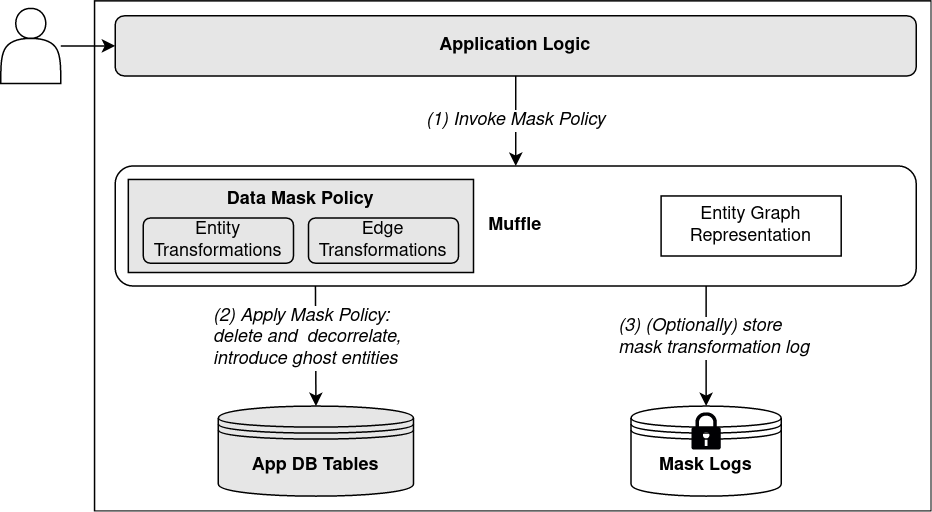
\includegraphics[width=0.5\textwidth]{img/muffle}

    \caption{High-level \sys architecture. Developers specify grayed-out components.}
    \label{fig:arch}
\end{figure}

\sys sits between the application logic and its database, and uses the developer mask policy to
model the application schema as an entity graph. \sys systematically applies the appropriate
mask transformations when invoked with the policy. 

If prompted, \sys will record the modifications performed during the transformation, and encrypts and
stores this log in an additional table. The encrypting key can be kept by the application for \eg content
moderation transformations, or in the case of user unsubscription, secret-shared~\cite{secretsharing}
among the user, \sys, and a trusted third party so that the user can retrieve a lost key without
trusting the application or \sys. To undo the transformation, \sys decrypts this log and reverses the
modifications, restoring the affected portion of the entity graph to its original state.

Figure~\ref{fig:arch} shows an example of a mask for user unsubscription, that supports reversing
the mask for resubscription.

\sys consists of 5K LoC of Rust, and supports SQL queries as well as \texttt{TRANSFORM
[entity\_id]} and \texttt{REVERSE TRANSFORM [entity\_id]} queries.
We show that \sys performs reasonably (Section~\ref{sec:perf}), and we plan to support eventually
consistent, crash-recoverable transformations, sharding, and multicore parallelism.

\iffalse
%-------------------------------------------------------------------------------
\section{Implementation}
%-------------------------------------------------------------------------------

\name introduces in-memory shim layer on top of a MySQL database, 
allowing \name to intercept and process queries sent by the application frontend. 
To amortize the cost of unsubscription and resubscription, \name preemptively creates, stores, and
links ghost parent entities to child entities if an update creates an edge that may be decorrelated.
\name builds in-memory materialized views on top of the underlying database, exposing ghost
entities only if the true entity has been decorrelated, and real entities otherwise. Updates
propagate to the materialized views when the underlying database is updated. \name answers
application queries using these materialized views, hiding the complexity of ghost entity and
decorrelation management.

\name is build in 5K LoC of Rust, and supports a subset of MySQL. \name adds \texttt{UNSUBSCRIBE
[user]} and \texttt{RESUBSCRIBE [user] WITH [user\_data]} calls to the query language.
\lyt{Should I mention details like query parsing, single-threaded?}

\subsection{Stored Data}
In addition to the original application data tables, \name stores a persistent mapping from entity
ID (EID) to a set of ghost IDs (GID). This mapping is cached in the shim layer for performance. Only
ghost entities that correspond to a true parent entity are stored in the mapping: auxiliary ghosts that are
created to introduce noise (reduce sensitivity), or to satisfy referential integrity---all their
children are also ghosts---are not linked to the real parent EID.

\name stores the in-memory materialized views for each datatable, using hashtables and btrees for
table indexes. An in-memory cache of the graph of parent-child entity key relationships built on
top of the views is also stored for unsubscription and resubscription performance.

Finally, \name stores a persistent and in-memory record of the hash of unsubscribed user EIDs 
and their removed application data to verify upon resubscription.

\subsection{Handling Normal Execution Queries}
\paragraph{Reads.}
Reads are answered by the materialized views. Because the materialized views are kept up-to-date with any application
writes, no queries to the underlying datatables are performed.
\lyt{I'm not sure if it's appropriate or interesting to put some of the MV query handling stuff
here? (Like processing joins, etc.)}

\paragraph{Inserts.}
When the application inserts an entity, \name first checks (using the developer-provided policy)
whether the entity is a child entity (i.e., it has a foreign key to another data table), and
whether the policy specifies that this child-parent key relationship should be decorrelated during
unsubscription. 

If so, \name preemptively creates a \emph{ghost parent} entity using the appropriate entity
generation policy, and adds this ghost to the parent data table. \name then saves the child
entity's real parent EID (the child entity's foreign key column value), and adds a mapping from this
EID to the new ghost parent GID.\footnote{\name assumes that the application does not violate
referential integrity, namely that any child entity inserted into the system will refer to a
corresponding parent in the database.} Finally, \name rewrites the child entity's foreign key
reference to correspond to this new ghost parent's GID, and stores the child into the datatable.

Note that generating the ghost parent may recursively generate a set of ghost ancestors for that
parent as well (to satisfy referential integrity). These ancestors are also added to the parent data
table.

The insert then propagates to the materialized view, inserting the entity with its real parent EID; queries that
select for this entity will not see any ghost entities. 

If the child-parent key relationship should not be decorrelated, or the inserted entity is not a
child, \name simply inserts the entity as-is into the datatable, and the materialized view is
updated with the entity.

\name also updates the parent-child entity graph with the new entity if the entity adds any edges
specified by the developer-provided policy. This graph is built on top of the materialized view, and
thus contains only those entities exposed by the materialized view to the application.

\paragraph{Updates.}
When the application updates an entity, \name again checks (using the developer-provided policy) whether
the entity is a child entity (i.e., it has a foreign key to another data table). 
If the entity is a child, and the policy specifies that this child-parent key
relationship should be decorrelated during unsubscription, then \name performs one final check of
whether the entity's parent key is one of the columns being updated.

If yes, then \name gets the current value of the entity parent key in the datatable: because \name
inserts only GIDs into the datatable for these decorrelatable child-parent links, this value 
corresponds to some ghost parent GID.
\name checks its ghosts mapping table for which real parent EID currently maps to this GID, removes
this current mapping, and updates the mapping so that the updated parent key value now points to
this GID.
\name updates all non-foreign key columns as normal, with values specified by the application.

If the updated entity is not a child of a decorrelatable edge, the update is performed without any
alterations.

Updates are propagated to the materialized view without modifying the values, so that application
reads only observe real parent entities.
\name also updates the parent-child entity graph if any edges between materialized view entities change.

\paragraph{Deletes.}
When the application deletes an entity, \name checks whether
the entity is a child entity (i.e., it has a foreign key to another data table). 
If the entity is a child, and the policy specifies that this child-parent key
relationship should be decorrelated during unsubscription, then \name gets the current value of the
entity parent key in the datatable, which must correspond to some ghost parent GID.
\name checks its ghosts mapping table for which real parent EID currently maps to this GID and removes
this mapping. \name also removes the ghost parent with this GID.

In all cases, \name removes the entity being deleted.
The deletion is propagated to the materialized view and removes the entity being deleted; the
parent-child entity graph is modified appropriately.

\subsection{Handling Unsubscription}
\paragraph{Traversal.}
\name is given the top-level entity type and EID to be decorrelated (typically a user and a user ID).
\name then performs a (depth-first) traversal of the parent-child entity graph built on top of the materialized
views. 

\name stores all the children entities traversed during decorrelation for post-processing, and
handles parent-child edges as follows:

If a parent-child edge has a no-decorrelation-retain policy, \name does nothing; if a parent child-edge has a
no-decorrelation-delete policy, \name removes the child entity and recursively removes all of its
descendants. 
\lyt{TODO: \name should apply the ghost generation policy to the parent node (replacing it with a ghost) for retain policies if a ghost generation policy exists.}

For every parent-child edge with a decorrelate policy, \name looks up the parent EID in the
EID to GIDs mapping, saves the corresponding GIDs, and removes the mapping (both persistent and
cached).
\name then updates the child entity in the materialized view to point to a ghost entity instead
than the real parent (who is being decorrelated) by choosing one of the corresponding GIDs for this
parent and updating the child's parent key with this GID.  The parent-child entity graph is updated
accordingly to include the ghost parent (note that this does not affect the traversal, which only
traverses parent-child edges).

If a parent-child edge has a no-decorrelation-sensitivity policy, \name stores the edge for
post-processing.

\paragraph{Sensitive Parent-Child Edges.}
Post-traversal, \name considers its collected set of sensitive edges. For every unique parent,
\name counts how many children attach to the parent for each distinct edge type (e.g,\ for a
particular tag, how many stories are linked to this tag, how many comments are linked to this tag,
etc.). For each child count $n$, and with an edge type sensitivity threshold of $\sigma$, 
\name generates $n / \sigma$ ghost entities of that child type, all of which have an edge to the parent.
These ghost entities are inserted both into the materialized views, and into the underlying
datatables; however, because they do not correspond to real entities, EID to GID mappings are not
stored. 
If \name finds no ghost generation policy for the child entity type, \name instead recursively
removes the child and its descendants.

\paragraph{Handling Child-Parent Edges.}
Next, \name considers child-parent edges from the collected set of traversed children to parents
not seen during \name's traversal. If an 
edge can be decorrelated, \name rewrites the materialized child parent key to one of the parent
ghost GIDs. The ghost GID is retrieved by querying the parent's EID to GIDs mapping, the
corresponding ghost parent is added to the materialized view,
and the mapping from parent EID to GID is subsequently removed. These steps ensure that the
materialized view reflects that the link between the child and the original parent has been
decorrelated.

If an edge has a delete policy, the child and its descendants are removed; if an edge has a retain
policy, nothing is done. 
%
\lyt{TODO: for retain policies, the ghost generation policy should be applied to the child node if
the ghost generation policy exists.}

If an edge $e$ has a senstivity threshold,
\name counts $N_{all}$, the total number of edges of the same edge type as $e$ that connect to $e$'s parent.
\name then counts $N_{sensitive}$, the number of these edges that connect to children that were traversed by \name during the
first decorrelation step (this number includes $e$).
If $e$'s edge type has sensitivity threshold of $\sigma$ and $N_{sensitive} / N_{all} > \sigma$,
\name generates $\lceil N_{sensitive}*\sigma\rceil - N_{all}$ ghost entities of $e$'s child type, all
of which have an edge to $e$'s parent.
As before, these ghost entities are inserted both into the materialized views, and into the underlying
datatables; however, because they do not correspond to real entities, EID to GID mappings are not
stored. 
If \name finds no ghost generation policy for the child entity type, \name instead recursively
removes the child and its descendants.

\paragraph{Decorrelated Entity Removal and Return Values.}
Finally, \name removes any completely isolated entities, namely any real entities that have no
descendants and are linked to only ghost (or no) parents. A completely isolated entity has either been swapped
out for a single ghost entity (in the case of a retained edge), or replaced by several ghost
entities, one per each decorrelated edge.

\name returns to the unsubscribing user (1) the removed parent EID to GIDs mappings, (2) any
completely isolated (and removed) entities,
and (3) the GIDs of any ghosts generated during sensitivity checks or to replace real
entities at the ends of retained edges.

To ensure that the end user cannot tamper with their application data while unsubscribed, \name saves
persistent and in-memory copies of the hash of the top-level entity EID and the returned data to
check upon resubscription.

\subsection{Handling Resubscription}
\name is given the top-level entity type and EID to be resubscribed, along with the data returned
from a prior unsubscription.
\name verifies that the hash of the EID and data matches that from the latest unsubscription of
this entity.

\name first re-inserts the completely decorrelated entities that were removed during unsubscription
into both the datatables and materialized views. 

Next, for all removed parent EID to GIDs mappings, \name reinserts these mappings into the
persistent and cached EID to GIDs mapping.
\name then removes the corresponding ghost entities for all GIDs and any ghost ancestors of these
GIDS from the materialized views; note that these ghosts still remain present in the
persistent data tables for future unsubscription.
\name then updates all materialized children of these removed ghosts with the original parent EID. Looking up the relevant
children is facilitated by the in-memory entity graph. 

Finally, \name removes any
ghost entities from the datatables and materialized views that were created during unsubscription to
lower sensitivity.

\subsection{Handling Crashes and Recovery}
Upon a crash, the in-memory materialized views are rebuilt from the underlying datatables and ghost
mapping. Any datatable entities without parents are simply reinserted into the appropriate
materialized view. 

If a datatable's entities have parent entities, the parent foreign keys may be ghost parent GIDs. 
This can happen for two reasons: 1) these child-parent edges can be decorrelated, and so ghost
entities had been preemptively created in the datatable; or 2) these are ghost entities created to
add noise to sensitive correlations during an unsubscription. 

For each entity with ghost parent GIDs, \name checks whether a mapping
from a real parent EID to the parent GID exists in the persistent EID to GIDs mapping. 
If such a mapping exists, then the real parent entity should be exposed to the application because
the parent or its ancestors have not yet unsubscribed: \name inserts the child entity with the real parent
EID into the materialized view.

Otherwise, if no mapping exists, then the ghost parent was generated during an unsubscription, and
the top-level entity has not yet resubscribed. \name thus exposes the ghost entity by inserting the
unmodified child entity with the parent GID into the materialized view.
Note that this may link a child entity with a \emph{different} ghost user than initially decided
during unsubscription (where any one of the ghosts corresponding to the real parent could be used as
a ghost parent for any child). 
\lyt{I think this can also be avoided by updating the MV entities with GIDs in monotonically
increasing order, since this is how they would have been inserted into the underlying database. It
also doesn't seem that important.}

The parent-child graph is constructed appropriately on top of the materialized view, and the EID to
GIDs mapping cache repopulated.

\lyt{TODO: Unsubscriptions and resubscriptions should be logged so that we can determine if they've
completed or not upon crashing. Eventual consistency for persistent / MV state in unsub/resub.}
\fi
